\documentclass{article}
\usepackage{tikz}
\usetikzlibrary{shapes.geometric, arrows}
\usetikzlibrary{shapes.misc, positioning}

\definecolor{lavander}{cmyk}{0,0.48,0,0}
\definecolor{violet}{cmyk}{0.79,0.88,0,0}
\definecolor{burntorange}{cmyk}{0,0.52,1,0}

\def\lav{lavander!90}
\def\oran{orange!30}

\tikzstyle{neighbors}=[draw,circle,violet,bottom color=\lav,
                  top color= white, font=\scriptsize,text=violet,minimum width=10pt]
\tikzstyle{queries}=[draw,circle,burntorange, left color=\oran,
                       text=violet,minimum width=30pt]

\tikzstyle{io} = [trapezium, trapezium left angle=70, trapezium right angle=110, minimum width=3cm, minimum height=1cm, text centered, draw=black, color=burntorange,left color=\oran]

\tikzstyle{process} = [rectangle, minimum width=3cm, minimum height=1cm, text centered, draw=black, bottom color=\lav, top color=white]

\tikzstyle{grey} = [ rectangle, rounded corners=10pt, bottom color=black!10, top color=black!2] 

\begin{document}
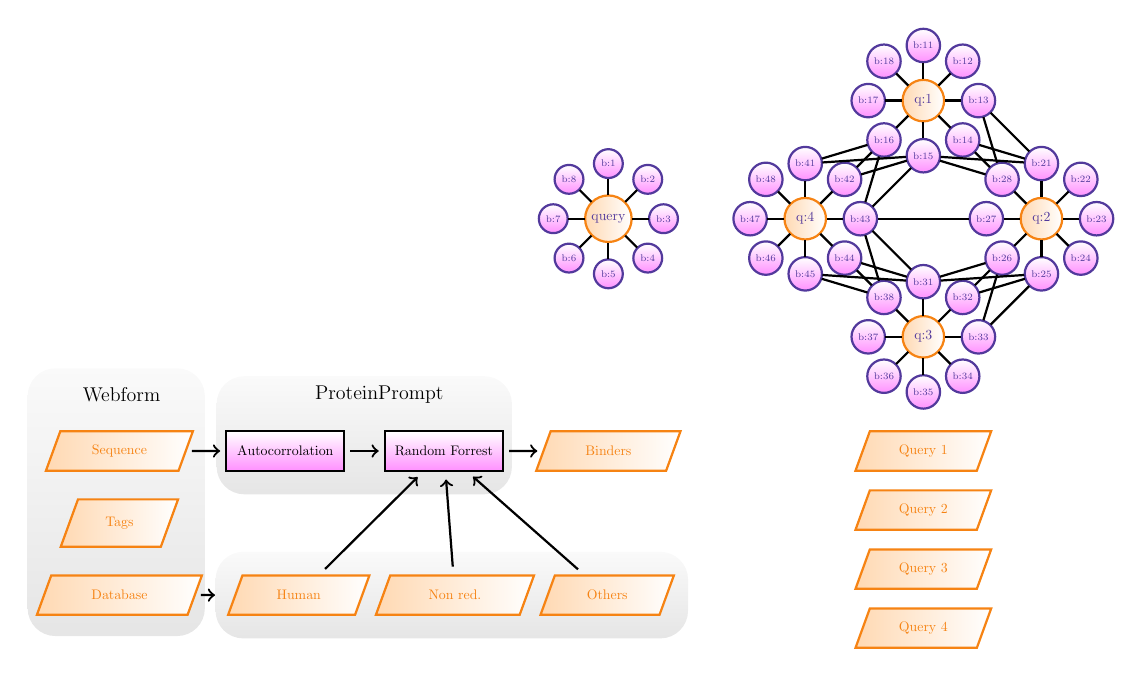
\begin{tikzpicture}[auto,thick, scale=0.5, transform shape,align=center, node distance = 1.5cm]

    \node[queries] (n0) at (-4,0) {query};
    \foreach \k/\l/\j in {1/1/2,-1/1/8,1.4/0/3,-1.4/0/7,1/-1/4,-1/-1/6,0/1.4/1,0/-1.4/5}{
        \node[neighbors] (n\j) at (\k-4,\l) {b:\j};
        %      \path (n\i\j) edge (\i);
        \draw (n\j) -- (n0);
    }
  \foreach \x/\y/\i in {1/0/4,7/0/2,4/3/1,4/-3/3} {
    \node[queries] (\i) at (\x,\y) {q:\i};
    \foreach \k/\l/\j in {1/1/2,-1/1/8,1.4/0/3,-1.4/0/7,1/-1/4,-1/-1/6,0/1.4/1,0/-1.4/5}{
        \node[neighbors] (\i\j) at (\x+\k,\y+\l) {b:\i\j};
        %      \path (n\i\j) edge (\i);
        \draw (\i\j) -- (\i);
    }
  }

  \foreach \i in {5,6}{
    \foreach \j in {1,2,3}{
      \draw (2\i) -- (3\j);
      \draw (1\i) -- (4\j);
    }
  }
  
  \foreach \i in {3,4,5}{
    \foreach \j in {1,8}{
      \draw (4\i) -- (3\j);
      \draw (1\i) -- (2\j);
    }
  }
  
  \draw (43) -- (27);


  

  \node (r1) [io, below of=35] {Query 1};
  \node (r2) [io, below of=r1] {Query 2};
  \node (r3) [io, below of=r2] {Query 3};
  \node (r4) [io, below of=r3] {Query 4};

  \node (webform) [grey, minimum width = 4.5cm, minimum height=6.8cm] at (-16.5cm,-7.2 ) {\parbox[t][5.8cm]{1.7cm}{\Large  Webform}};

  \node (server) [grey, minimum width = 7.5cm, minimum height=3cm] at (-10.2cm,-5.5 ) {\parbox[t][2.5cm]{2.5cm}{\Large  ProteinPrompt}};

  \node (result) [io] at (n5 |- r1) {Binders};

  \node (prompt) [process, left=1cm of result] {Random Forrest};

  \node (ac) [process, left=1cm of prompt] {Autocorrolation};

  \node (seq) [io, left=1cm of ac] {Sequence};
  \node (tag) [io, below=0.7 of seq] {Tags};
  \node (db)  [io, below=0.7 of tag] {Database};


  \node (backdb) [grey, right=0.5cm of db, minimum width=12cm, minimum height=2.2cm] {};
  
  \node (db1) [io, right=1cm of db] {Human};
  \node (db2) [io, right=0.5cm of db1] {Non red.};
  \node (db3) [io, right=0.5cm of db2] {Others};

  \draw [->, shorten >=2pt, shorten <=2pt] (seq) -- (ac);
  \draw [->, shorten <=2pt] (db) -- (backdb);
  \draw [->, shorten >=2pt, shorten <=2pt] (ac) -- (prompt);
  \draw [->, shorten >=2pt, shorten <=2pt] (prompt) -- (result);
  \draw [->, shorten >=3pt, shorten <=3pt] (db1) edge (prompt);
  \draw [->, shorten >=3pt, shorten <=3pt] (db2) edge (prompt);
  \draw [->, shorten >=3pt, shorten <=3pt] (db3) edge (prompt);
  
\end{tikzpicture}
\end{document}
